
%% bare_conf.tex
%% V1.3
%% 2007/01/11
%% by Michael Shell
%% See:
%% http://www.michaelshell.org/
%% for current contact information.
%%
%% This is a skeleton file demonstrating the use of IEEEtran.cls
%% (requires IEEEtran.cls version 1.7 or later) with an IEEE conference paper.
%%
%% Support sites:
%% http://www.michaelshell.org/tex/ieeetran/
%% http://www.ctan.org/tex-archive/macros/latex/contrib/IEEEtran/
%% and
%% http://www.ieee.org/

%%*************************************************************************
%% Legal Notice:
%% This code is offered as-is without any warranty either expressed or
%% implied; without even the implied warranty of MERCHANTABILITY or
%% FITNESS FOR A PARTICULAR PURPOSE! 
%% User assumes all risk.
%% In no event shall IEEE or any contributor to this code be liable for
%% any damages or losses, including, but not limited to, incidental,
%% consequential, or any other damages, resulting from the use or misuse
%% of any information contained here.
%%
%% All comments are the opinions of their respective authors and are not
%% necessarily endorsed by the IEEE.
%%
%% This work is distributed under the LaTeX Project Public License (LPPL)
%% ( http://www.latex-project.org/ ) version 1.3, and may be freely used,
%% distributed and modified. A copy of the LPPL, version 1.3, is included
%% in the base LaTeX documentation of all distributions of LaTeX released
%% 2003/12/01 or later.
%% Retain all contribution notices and credits.
%% ** Modified files should be clearly indicated as such, including  **
%% ** renaming them and changing author support contact information. **
%%
%% File list of work: IEEEtran.cls, IEEEtran_HOWTO.pdf, bare_adv.tex,
%%                    bare_conf.tex, bare_jrnl.tex, bare_jrnl_compsoc.tex
%%*************************************************************************

% *** Authors should verify (and, if needed, correct) their LaTeX system  ***
% *** with the testflow diagnostic prior to trusting their LaTeX platform ***
% *** with production work. IEEE's font choices can trigger bugs that do  ***
% *** not appear when using other class files.                            ***
% The testflow support page is at:
% http://www.michaelshell.org/tex/testflow/



% Note that the a4paper option is mainly intended so that authors in
% countries using A4 can easily print to A4 and see how their papers will
% look in print - the typesetting of the document will not typically be
% affected with changes in paper size (but the bottom and side margins will).
% Use the testflow package mentioned above to verify correct handling of
% both paper sizes by the user's LaTeX system.
%
% Also note that the "draftcls" or "draftclsnofoot", not "draft", option
% should be used if it is desired that the figures are to be displayed in
% draft mode.
%
\documentclass[conference]{IEEEtran}
% Add the compsoc option for Computer Society conferences.
%
% If IEEEtran.cls has not been installed into the LaTeX system files,
% manually specify the path to it like:
% \documentclass[conference]{../sty/IEEEtran}





% Some very useful LaTeX packages include:
% (uncomment the ones you want to load)


% *** MISC UTILITY PACKAGES ***
%
%\usepackage{ifpdf}
% Heiko Oberdiek's ifpdf.sty is very useful if you need conditional
% compilation based on whether the output is pdf or dvi.
% usage:
% \ifpdf
%   % pdf code
% \else
%   % dvi code
% \fi
% The latest version of ifpdf.sty can be obtained from:
% http://www.ctan.org/tex-archive/macros/latex/contrib/oberdiek/
% Also, note that IEEEtran.cls V1.7 and later provides a builtin
% \ifCLASSINFOpdf conditional that works the same way.
% When switching from latex to pdflatex and vice-versa, the compiler may
% have to be run twice to clear warning/error messages.






% *** CITATION PACKAGES ***
%
% \usepackage{cite}
% cite.sty was written by Donald Arseneau
% V1.6 and later of IEEEtran pre-defines the format of the cite.sty package
% \cite{} output to follow that of IEEE. Loading the cite package will
% result in citation numbers being automatically sorted and properly
% "compressed/ranged". e.g., [1], [9], [2], [7], [5], [6] without using
% cite.sty will become [1], [2], [5]--[7], [9] using cite.sty. cite.sty's
% \cite will automatically add leading space, if needed. Use cite.sty's
% noadjust option (cite.sty V3.8 and later) if you want to turn this off.
% cite.sty is already installed on most LaTeX systems. Be sure and use
% version 4.0 (2003-05-27) and later if using hyperref.sty. cite.sty does
% not currently provide for hyperlinked citations.
% The latest version can be obtained at:
% http://www.ctan.org/tex-archive/macros/latex/contrib/cite/
% The documentation is contained in the cite.sty file itself.





\usepackage[dvips]{graphicx}
\graphicspath{{./images/}}
\DeclareGraphicsExtensions{.eps,.bmp}

\hyphenation{op-tical net-works semi-conduc-tor}


\begin{document}
%
% paper title
% can use linebreaks \\ within to get better formatting as desired
\title{An Analysis of Highspeed Interconnect Technology: Quickpath
Interconnect, PCI-Express and HyperTransport}


% author names and affiliations
% use a multiple column layout for up to three different
% affiliations
\author{\IEEEauthorblockN{James Swaro}
\IEEEauthorblockA{School of Electrical Engineering\\ and Computer Science\\
Ohio University\\
Athens, Ohio 45701--3241\\
Email: js311004@ohio.edu}
}

% make the title area
\maketitle


\begin{abstract}
\label{sec:abstract}
%\boldmath
This paper serves to evaluate Quickpath Interconnect, HyperTransport and PCI
Express as highspeed interconnect technologies. A comparison will be made,
highlighting the advantages and disadvantages of each technology. Quickpath
Interconnect is a proprietary technology developed by Intel to increase the
available bandwidth between the CPU and the north bridge. PCI-Express is
technology managed by PCISIG that serves as a replacement for PCI and PCI-X,
while also attempting to be a consumer grade highspeed motherboard--level
interconnect. HyperTransport is an interconnect technology designed by AMD
designed to functionas a direct to CPU interconnect for I/O devices. This paper
will summarize each technology in detail, comparing the advantages and
disadvantages of each technology as well as a brief synopsis about how each
interconnect functions. 
\end{abstract}
% IEEEtran.cls defaults to using nonbold math in the Abstract.
% This preserves the distinction between vectors and scalars. However,
% if the conference you are submitting to favors bold math in the abstract,
% then you can use LaTeX's standard command \boldmath at the very start
% of the abstract to achieve this. Many IEEE journals/conferences frown on
% math in the abstract anyway.

% no keywords




% For peer review papers, you can put extra information on the cover
% page as needed:
% \ifCLASSOPTIONpeerreview
% \begin{center} \bfseries EDICS Category: 3-BBND \end{center}
% \fi
%
% For peerreview papers, this IEEEtran command inserts a page break and
% creates the second title. It will be ignored for other modes.
\IEEEpeerreviewmaketitle



\section{Introduction}
\label{sec:intro}
% no \IEEEPARstart
As computers are increasing in performance in the areas of memory, networking,
storage and processing, the interconnects must also improve. The improvement of
interconnects comes as a necessity so that overall systems performance does not
become hindered as other components improve. Such components include the
processor, memory and I/O devices which are constantly increasing in bandwidth,
the interconnects that connect these devices must also improve. 
In modern computers, the northbridge typically serves as the interconnect fabric
between the southbridge, graphics and memory hub to the processor. The
southbridge is responsible for communicating with slower I/O devices and the
north bridge. However, in high performance computing, it can be easy to find
that the bandwidth required to perform certain tasks can exceed that of the
available bandwidth. This is where it is often necessary to look at faster
interconnect technologies such as HyperTransport, QPI or PCI-Express. 

Each technology addresses the need for faster I/O with the CPU in a different
way. The way in which this is done can vary greatly with each technology and
with differing results. This paper will address the differences between each
technology and examine the advantages versus the disadvantages of each
technology to provide an unbiased analysis. 

\section{QuickPath Interconnect}
\subsection{Overview}
\subsection{How does it operate?}
\subsection{Advantages}
\subsection{Disadvantages}


\section{HyperTransport}
\label{sec:ht}

\subsection{Overview}
\label{subsec:ht:over}
HyperTransport was originally designed to support to need simplify high-speed
data traffic between memory, I/O or the processor. The first
specification, HyperTransport 1.03 defined a bandwidth of up
to 12.8 GB/s aggregate bandwidth.\cite{htWhitePaper} HyperTransport 2.0
supports 22.4 GB/s aggregate bandwidth and the newest specification,
HyperTransport 3.10 supports up to 25.6GB/s unidirectional.

HyperTransport is refered to as a ``mezzanine connector from a system's main
processor or memory controller to another I/O, often a PCI bus, within the
system, perhaps for additional chip or component.''\cite{paulson2003ins} As I
have read, HyperTransport is often directly connected to the CPU and functions
similarly to the northbridge but only for highspeed I/O devices. 

HyperTransport is a point-to-point link technology that uses two seperate
point-to-point links for bi-directional traffic, up to speeds of 51.2GB/s
bidirectional. A set of HyperTransport links can be seen in Figure
\ref{fig:htLinks}. 

\begin{figure}[!t]
	\begin{center}
		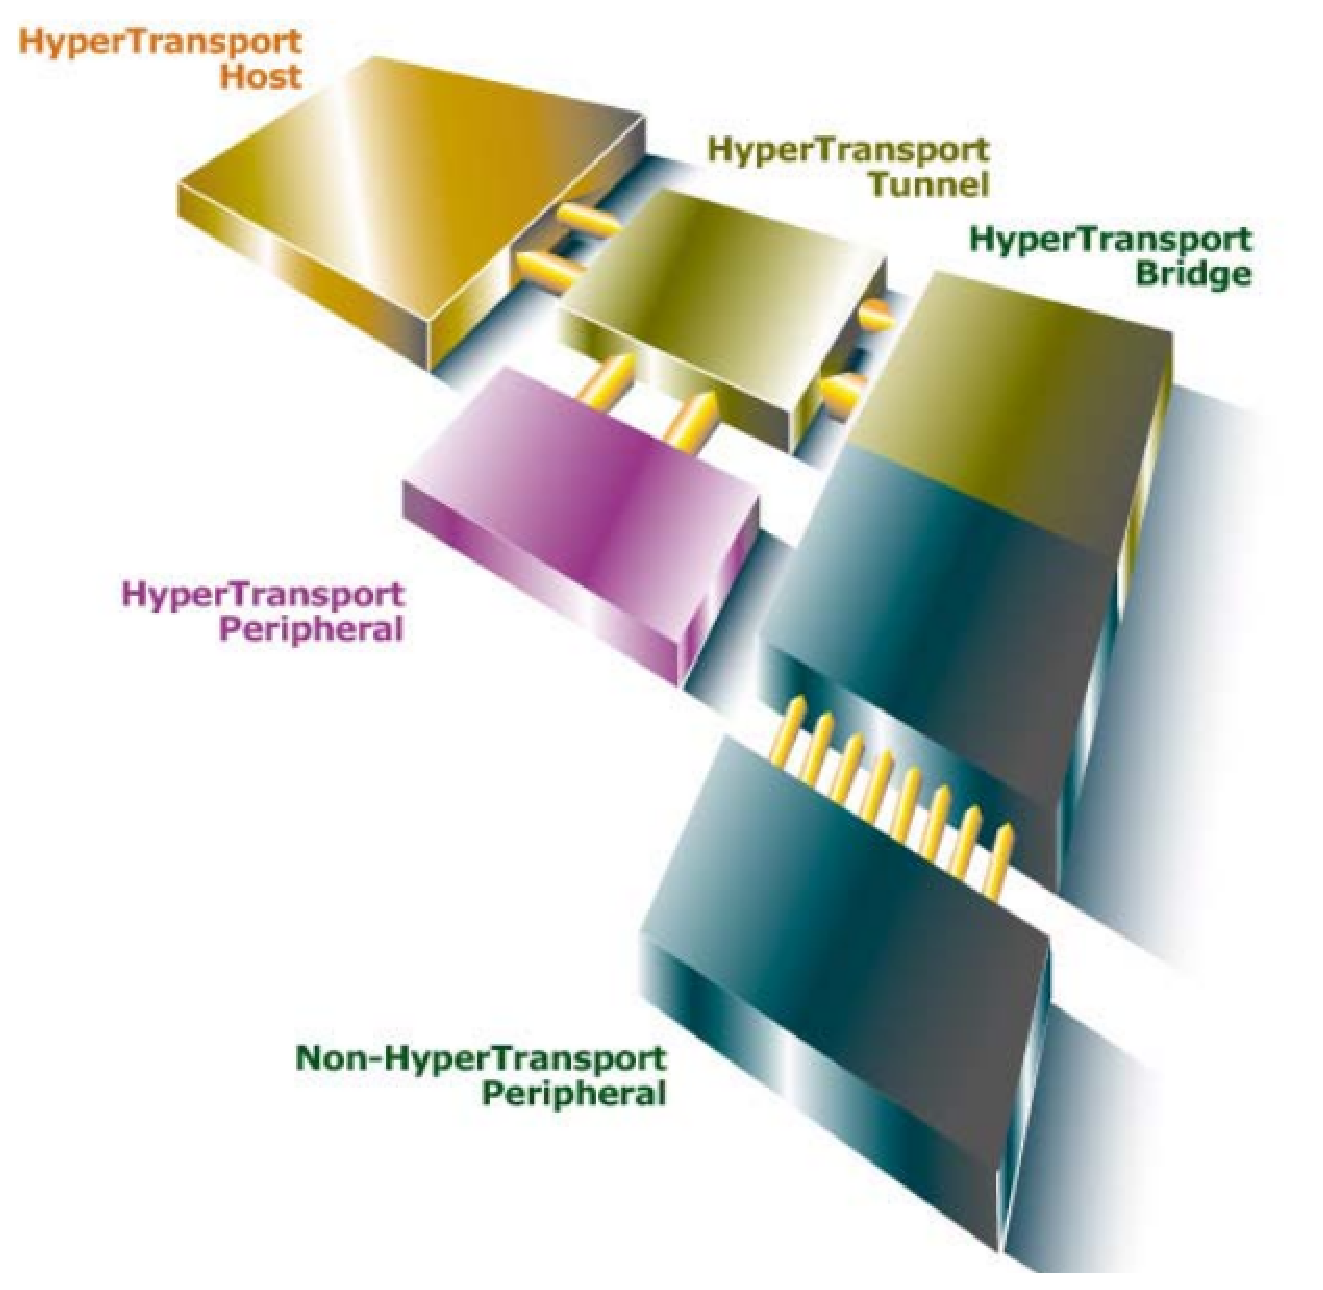
\includegraphics[scale=.35]{htLinks}
	\end{center}
	\caption{
	 The HyperTransport Link consists of at least one host (often a
	 HyperTransport-enabled CPU) and one tunnel/endpoint. A tunnel enables the
	 HyperTransport link to be passed from one HyperTransport-enabled device to
	 another in daisy-chain fashion.
	\cite{htWhitePaper}\label{fig:htLinks}}
	\label{fig:ht:packet}
\end{figure}

HyperTransport is also a very low latency protocol with a very high bandwith
capability. It is achieved by the following:\cite{duato2009extending}

\begin{itemize}
  \item Minimizing packet overhead
  \item Eliminating control and command signals needed by other protocols
  \item Reducing crosstalk and interference
\end{itemize}

HyperTransport is however primarily a host-to-host or host-to-I/O protocol.
This can be observed in Figure \ref{fig:ht:diagram}. It does not see that same
benefits as it is expanded to larger scale environments. HyperTransport interconnects can function as a replacement of the
northbridge,  a multiprocessor interconnect or a switch bus. 
HyperTransport has four different protocol versions. HT protocol 1.x and 2.0
are clock-forwarded interface types. The links are considered to be
uni-directional reliable links, operating at a clock speed of 200 Mhz to 3.2Mhz(HT3.1).
HyperTransport 3.0 and up is not considered to be reliable due to the use of
data recovery techniques.\cite{holden2006latency}. However, it can be shown that
the rate of bit errors is low. 

HyperTransport was designed to be an extremely low latency protocol. With this
in mind, the designers created HyperTransport in such a way as to minimize the
latency within the physical, data link and transaction layer. This is due to
the low amount of packet overhead generated by the headers in a HT packet and a
skew-constrained PCB.

\begin{figure}[!t]
	\begin{center}
		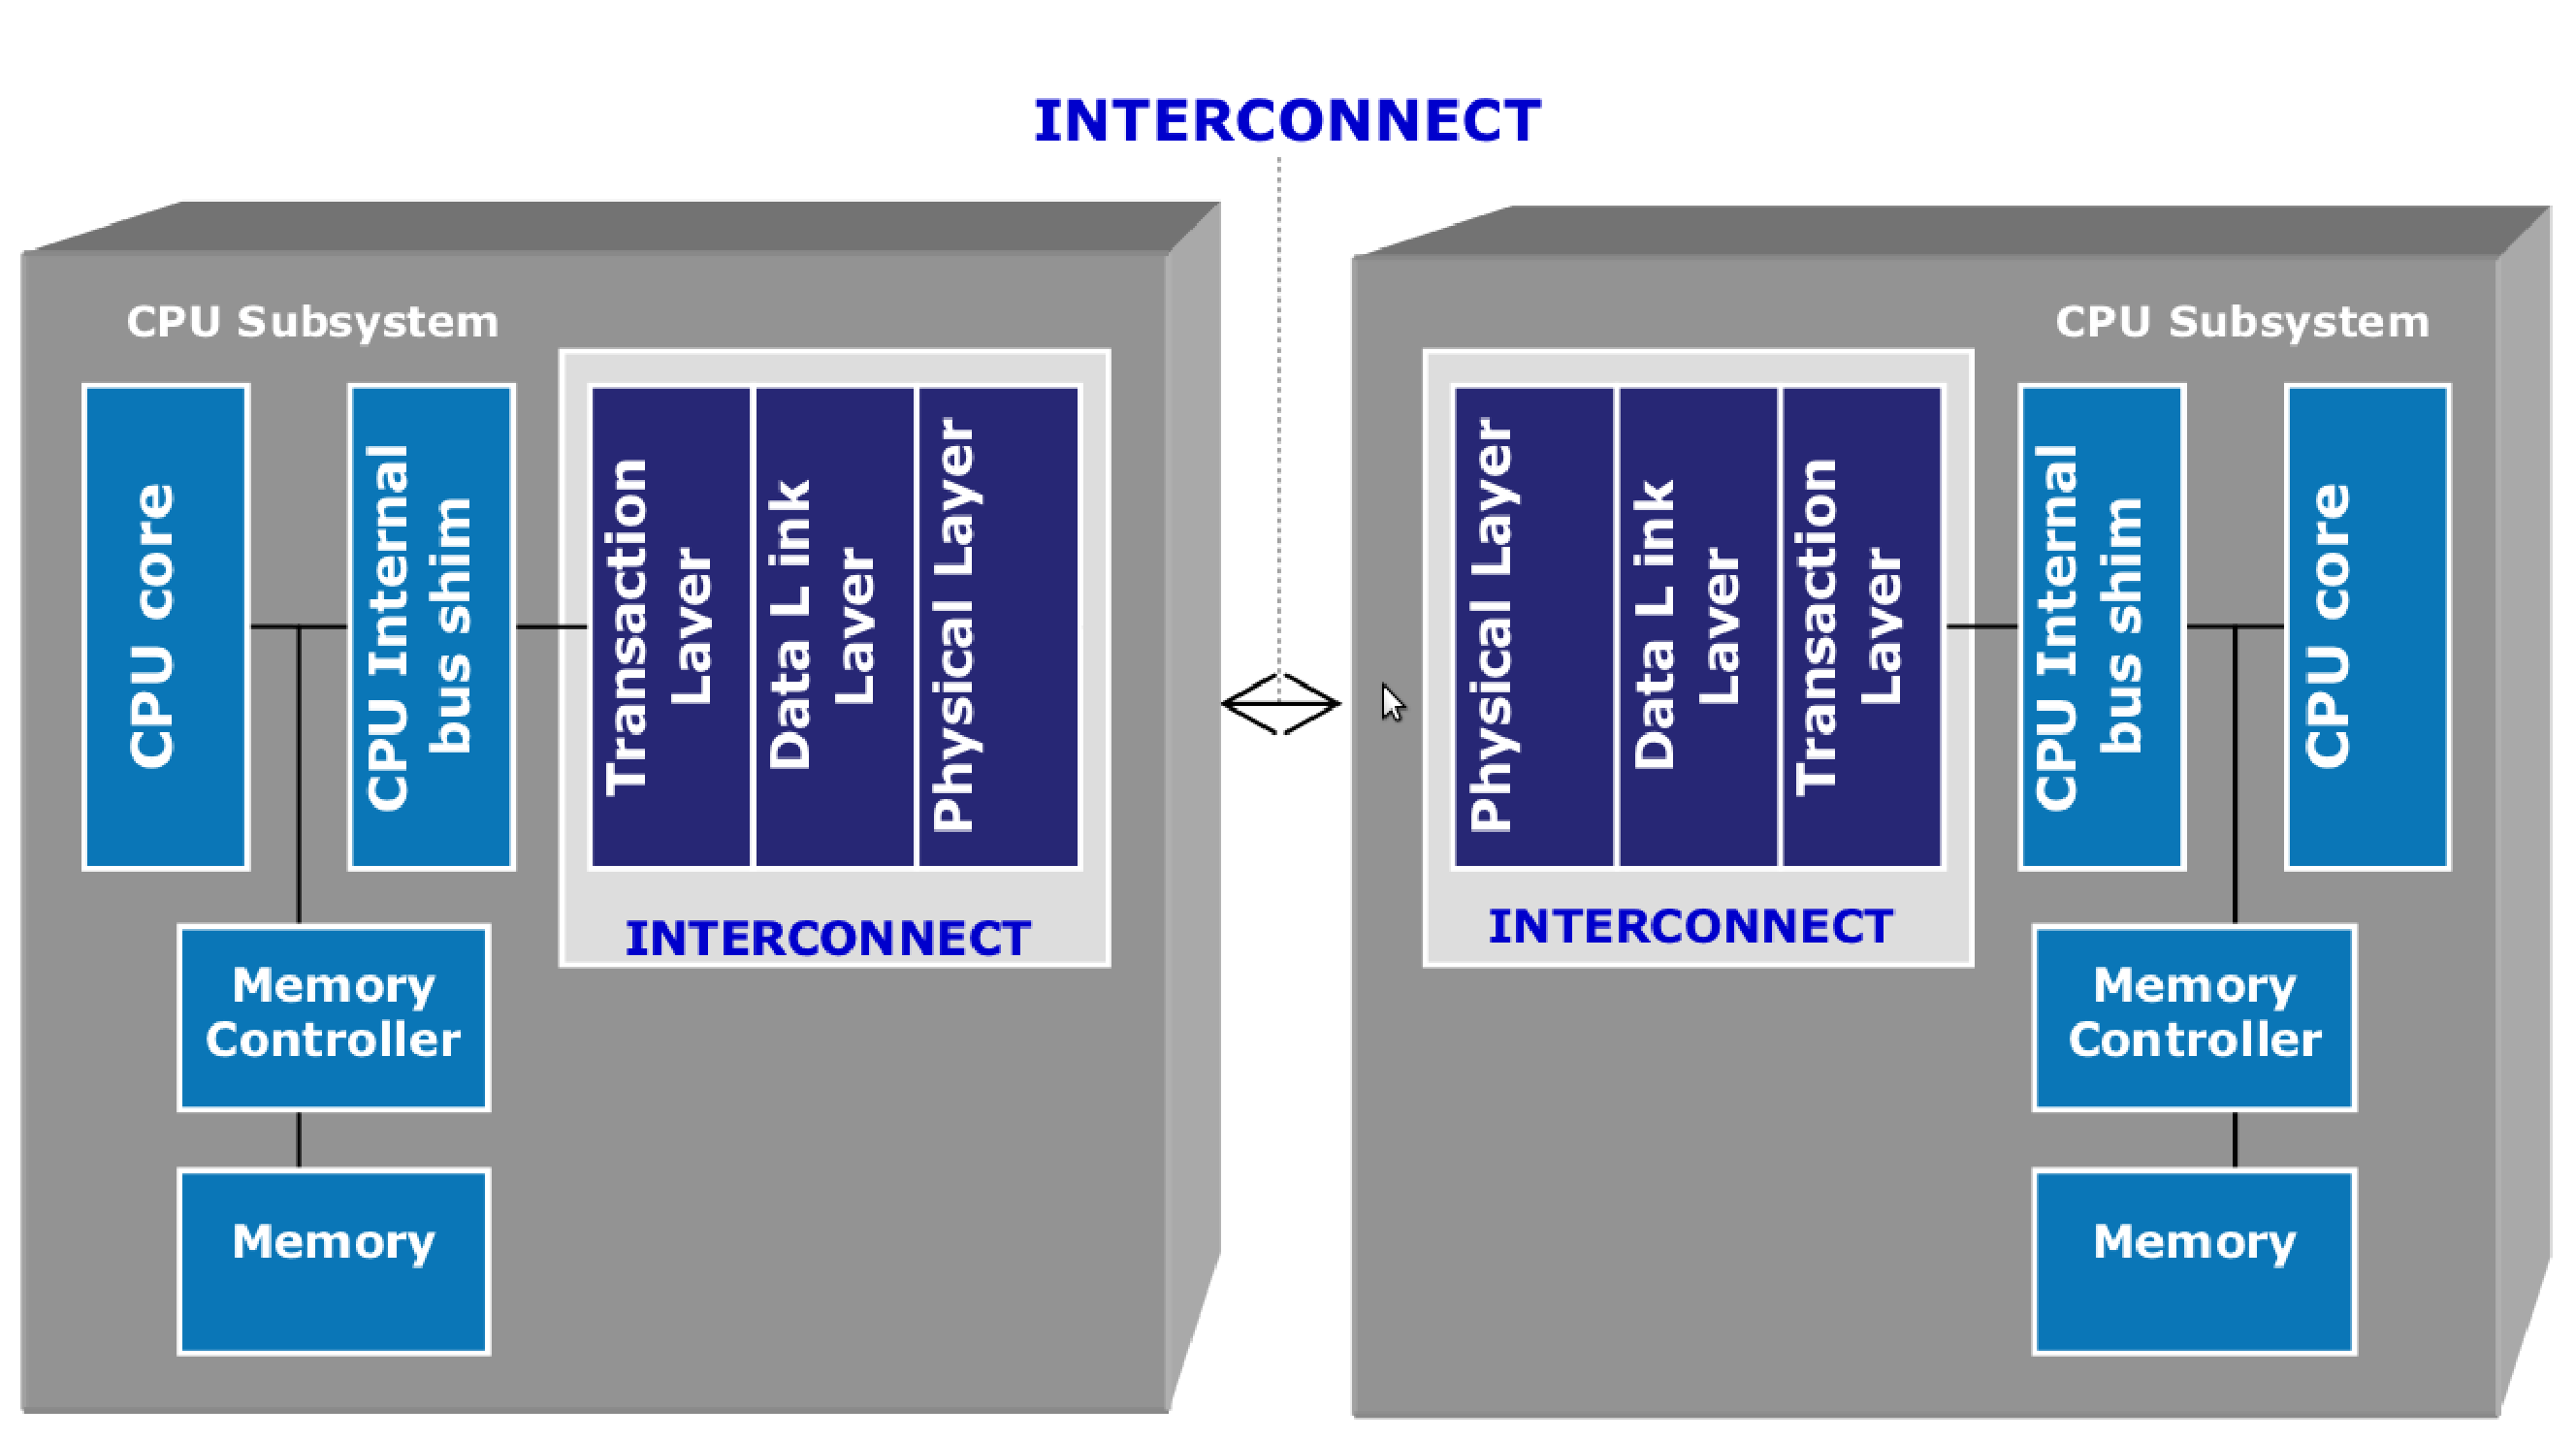
\includegraphics[scale=.15]{htDiagram}
	\end{center}
	\caption{point-to-point visualization of a
	HyperTransport link.\cite{holden2006latency}.}
	\label{fig:ht:diagram}
\end{figure}

\subsection{How does it operate?}
\label{subsec:ht:oper}


HyperTransport is often connected directly to the CPU. It serves as a bridge
between highspeed I/O devices and the CPU providing a high bandwidth channel for
multiple devices to use to communicate. Each devices is connected to the HT bus
through a daisy chain. Up to thirty-two devices to be connected to any single
daisy chain. The daisy chain operates by allowing a device to take up a set of lines,
of which do not have to match the number of lines taken by other devices. For
example, a single I/O devices connected to the HT unit, can utilize two lines,
while another device can use eight. 

The HT protocol maintains the high speed by eliminating overhead from packets
transfered. The read packets of a HT link only have an overhead of eight bytes
while the write packets have an overhead of twelve bytes. This minimal amount of
bytes reserved for overhead results in a large boost in performance. This can be
observed in Figure \ref{fig:ht:packet}.

\begin{figure}[!t]
	\begin{center}
		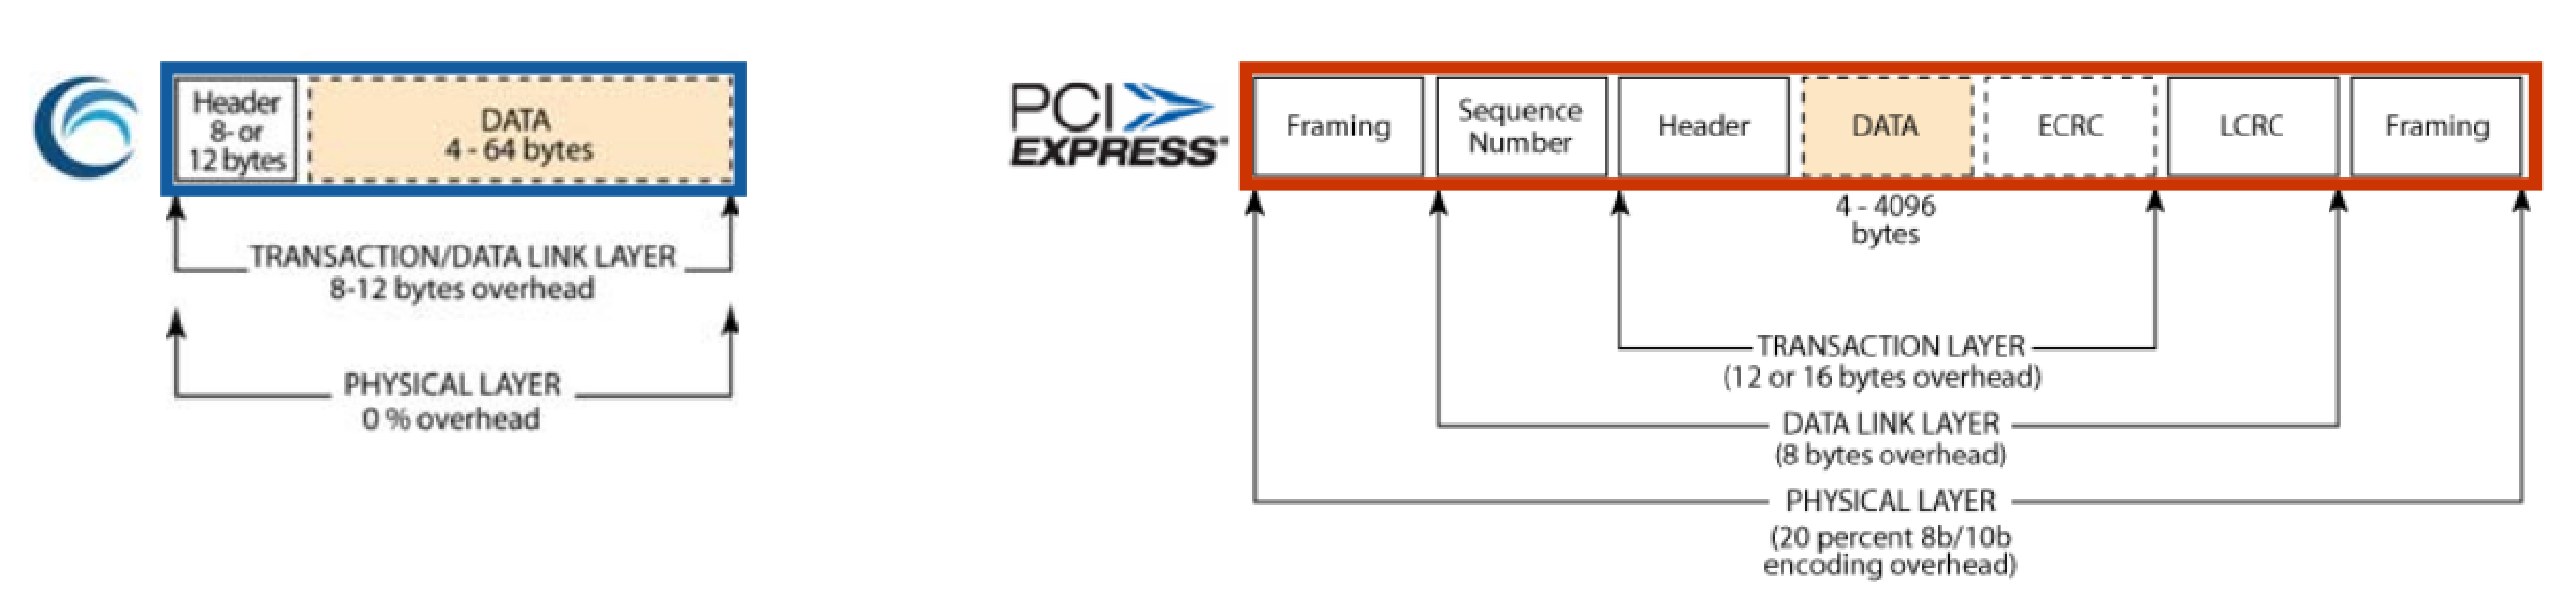
\includegraphics[scale=.2]{htPacket}
	\end{center}
	\caption{A comparison between a HyperTransport packet and a PCI-Express
	packet.\cite{holden2006latency}}
\end{figure}
 
\subsection{Advantages}
\label{subsec:ht:advant}
HyperTransport is designed with many key advantages in mind. The interface
design for HyperTransport 1.x and 2.0 is considered to be inherently reliable.
This improves throughput as less effort is expended attempting to retransmit
lost data. It is further improved upon by looking at the bit error ratio.
HyperTransport consortium claims that the bit-errror-ratio of the system is
often 10-15 or better.\cite{holden2006latency} This allows the designers to use
simple error detection instead of complicated and often expensive in terms of either latency or
bandwidth loss. 

Low latency is a key design advantage that was considered during the development
of HyperTransport. With that in mind, Priority Request Interleaving is a feature
specific to HyperTransport that allows for data to be halted and control packets
to be inserted in the case where a control packet may need to be transmitted
immediately. This is significant in that PRI can reduce latency considerably,
usually in response to a cache-miss or similar events\cite{holden2006latency}.

Consider the following event given from the Latency Comparison paper from
the HyperTransport Consortium:

\quote{While data transfer 1 is underway between peripheral B and the host, the need arises for
peripheral A to start a data transfer from the host. Without PRI, transfer 2 would have to wait
until transfer 1 completes and, should transfer 1 be the answer to a cache miss, for instance,
latency for transfer 2 would become prohibitive. With PRI, a control packet is promptly
inserted within transfer 1's data stream, instructing the link to initiate data transfer 2 on the
other link channel concurrently with the completion of data transfer 1. This mechanism,
unique to HyperTransport technology, greatly reduces latency of HyperTransport-based
systems.}\cite{holden2006latency}

HyperTransport also does split-phase transactions that allow the I/O device to
continue on with other tasks. In addition, HyperTransport does not require framing or coding at the physical
layer, CRC is performed every 512 bytes instead of a packet by packet basis and
no data link layer packet overhead is present.

\subsection{Disadvantages}
\label{subsec:ht:disadv}
Unfortunately, HyperTransport does not support hardware error recovery at the
link layer. The following is a list of things that HyperTransport cannot do
well:

\begin{itemize}
  \item Cannot do global device addressing beyond 32 nodes.
  \item Efficient routing in scalable network topologies
  \item Scalable congestion management mechanisms
  \item Dynamic reconfiguration of routing information
\end{itemize}

The above items are relevant for clustering HyperTransport devices in medium to
large clusters of processing nodes\cite{duato2009extending}. 

\section{PCI-Express}
\subsection{Overview}
PCI-Express was designed by PCISIG as an upgrade to the old PCI and PCI-X
technologies. As the necessity for higher bandwidth to support I/O devices rose, the need for faster interconnect
initiated the design of PCI-Express. PCI-Express is a switched, serial
interconnect technology. PCI-Express serves as a switch environment to a
plethora of I/O devices ranging from graphics to highspeed I/O devices like
networking interfaces. The architecture is layered similarly to the OSI
technology and it is designed to be compatible with copper, optical or other
forms of media\cite{paulson2003ins}. PCI-Express allows for hot-plugging and
power management. Originally known as 3GIO, PCI-Express has been in development
for a long time with PCI-Express 3.0 being the latest standard with PCI-Express
4.0 under development and slated for 2014/15 specification release date. 

Functionally, PCI and PCI-Express are both bus topologies. PCI is a shared bus
technology where PCI-Express is a point-to-point bus technology where each
device has a seperate serial link connecting it to the root complex of the PCI
Express bus.\cite{budruk2004pci} The structure of a PCI-Express interconnect can
be observed in Figure \ref{fig:pci:diagram}.

\begin{figure}[!t]
	\begin{center}
		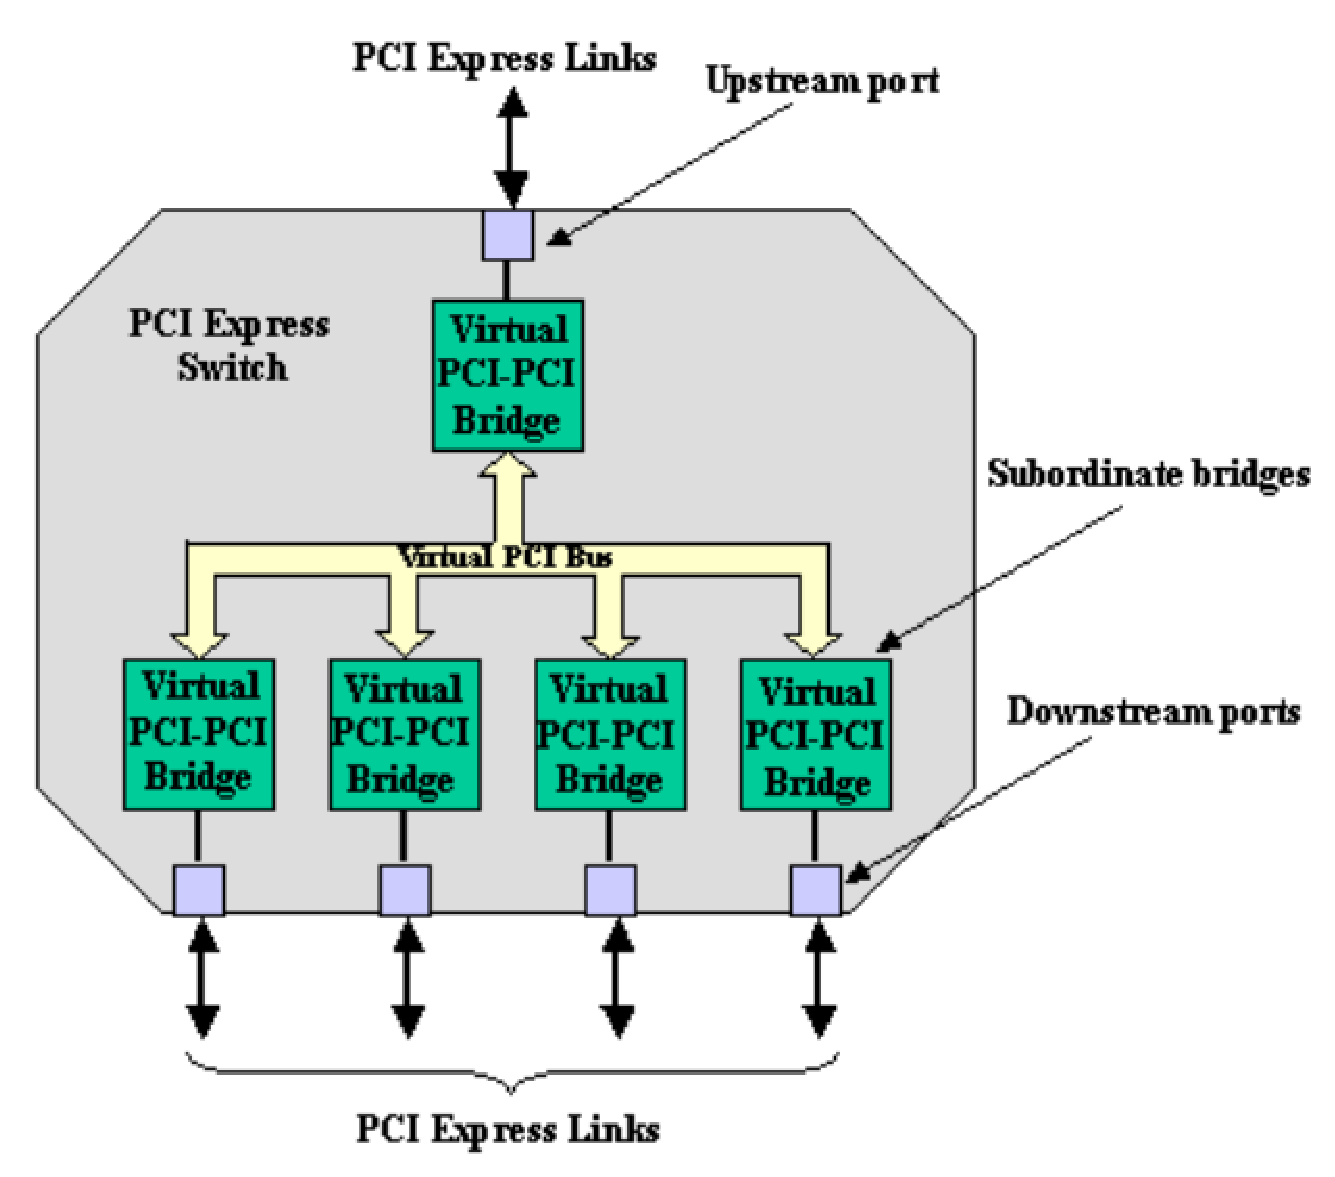
\includegraphics[scale=.4]{pciDiagram}
	\end{center}
	\caption{PCI Express Architecture as it functions as a switching fabric
	between highspeed I/O devices.\cite{mayhew2003pci}}
	\label{fig:pci:diagram}
\end{figure}

The PCI-Express link between any two devices can consist of one to thirty-two
lanes. A lane is a set of Tx/Rx Pair of lines connecting two devices, creating
a full duplex environment in which packets are transported. To expand upon this,
PCI-Express also allowed the data to be delivered in parallel on connections in
which more than one lane exists.The current specification, PCI-Express 3.0 can
do 8.0GT/s or 16GB/s in a sixteen-lane environment. 

PCI-Express is considered to be an ``inside of the box'' I/O solution while
other technologies such as infiniband can be used to connect highspeed devices
or cluster interconnects.

\subsection{How does it operate?}
\label{sub:pci:oper}
PCI-Express is a multi-drop, parallel bus topology. Each interconnect contains a
Host bridge and has several endpoints to connect I/O
devices\cite{bhatt2003creating}. PCI-Express functions on three different layers
of the OSI model, mapped to the Physical layer, Data link layer and Transaction
layer. The Data transmission layer is responsible for sending all control
messages, interrupts and data for the interconnect. Data is interleaved such
that each successive byte is sent down each successive lane available to the
connection. This is how the connection between devices is parallelized to
increase bandwidth between devices. 

The data is encoded in a 8b to 10b transfer
encoding, creating a twenty percent overhead at the Physical layer. An
improvement was made in PCI-Express 3.0 such that the data was encoded in a 128b
to 130b transfer encoding, decreasing the overhead incurred at the Physical
layer of the protocol.

The data link layer was designed to ensure the reliable deliver of packets
between two endpoints using ACK/NACK and a sliding window. PCI-Express also
utilizes a credit-based flow control that always ensures that there is space for
the packets sent in the next hop of the path.

The Transaction layer utilizes split transactions similar to HyperTransport
allowing I/O devices to continue other tasks while waiting for read and write
requests to complete. This layer will generate the read and write requests and
pass down to the data link layer for the addition of sequence information and
CRC checking. 



\subsection{Advantages}
\subsection{Disadvantages}

\section{Technology Comparisons}
\subsection{HyperTransport Vs. PCI-Express}

\subsection{HyperTransport Vs. QuickPath Interconnect}


\subsection{PCI-Express Vs. QuickPath Interconnect}

\subsection{Overall Breakdown}

\section{Conclusion}

\section*{Acknowledgment}
The authors would like to thank...

\bibliographystyle{IEEEtran}
\bibliography{IEEEabrv,kodiTermPaper}
\end{document}


